% NOTE: Sciposter is dependent on the following packages: a0size, boxedminipage, color,
% graphics, ifthen, shadow, times
% You need to have these packages installed for for sciposter to run properly

\documentclass[landscape,26pt]{sciposter}

%%% Document Class Options %%%%
%portrait		% The default, orients paper in portrait mode
%landscape 		% Orients paper in landscape mode		
%boxedsections	% The default, makes section titles appear in boxes
%ruledsections	% Makes section titles appear underlined
%plain sections	% Makes section titles appear plain 


\usepackage{epsfig}
\usepackage{amsmath}
\usepackage{amssymb}
\usepackage{multicol}
\usepackage{wallpaper}
\usepackage{rotating}
\usepackage{verbatim}
\usepackage{epstopdf}
\usepackage{sidecap}
%\usepackage{pstricks}
%\usepackage{caption}
%\usepackage{subcaption}

\newtheorem{Def}{Definition}
\renewcommand{\titlesize}{\huge}
\renewcommand{\authorsize}{\Large}
\renewcommand{\instsize}{\large}
\renewcommand{\sectionsize}{\large}
\title{Controller for Jumping Animations to Achieve Target Position}

% The author's or authors' names
\author{\ \\ Ian Ooi and Barbara Cutler}
 
% insert correct institute name
\institute{Department of Computer Science\\
           Rensselaer Polytechnic Institute\\}

\email{ooii@rpi.edu,cutler@cs.rpi.edu}  % shows author email address below institute

\leftlogo{logos/lgpseal.eps}
\rightlogo{logos/logo_cs_design_1.png}

%\setlength{\wpXoffset}{-30in}
%\setlength{\wpYoffset}{-32.2in}
%%%%%%%%%%%%%%%%%%%%%%%%%%%%%%%%%%%%%%%%%%%%%%%%%%%%%%%%%%%%%%%%%%%%%%%%%%%%%%%%
\begin{document}
%%%%%%%%%%%%%%%%%%%%%%%%%%%%%%%%%%%%%%%%%%%%%%%%%%%%%%%%%%%%%%%%%%%%%%%%%%%%%%%%


\maketitle

\begin{minipage}[t]{10.5in}
	\section*{Overview}
		We describe a controller for the generation of plausible human jumping motions with a forward physics based simulation.  Jumping is described as the acceleration of a character's center of mass to achieve upward motion, with the character breaking contact with the ground.  The motion is further divided into several stages of a windup or lead-up in which the character prepares to accelerate their center of mass, an acceleration stage in which the character applies a force to accelerate upward to leave the ground, an in-air stage in which the character is airborne, and finally landing.  We develop this controller in a modular manner, allowing it to be composed with other controllers to create complex compound motions, focusing on the stages before the character is in the air.  The controller models the muscles as springs which produce forces on the limbs of the leg.  Force is distributed to different springs, with joints bent to not only gain potential energy in the springs but to also to maintain balance.  Balance is maintained by positioning the center of mass over the supporting polygon formed by the character's feet.

		\vspace{.3in}

	\section*{Background and Motivation}
        Animations for video games and other entertainment applications are usually produced manually by an artist, then played back at appropriate times.  They are specified by keyframes, selected important frames where a static pose of a 3D model is set.  Interpolation is performed between these frames to produce a smooth animation.  This process is work intensive and lacks flexibility, requiring artists to manually set many poses for 3D models.
		\begin{figure}
			\centering
            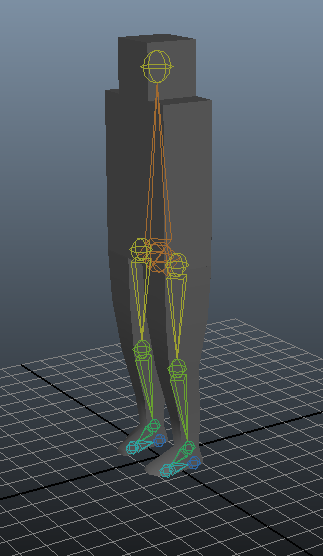
\includegraphics[height=5in]{skel_example/skel1.png}
            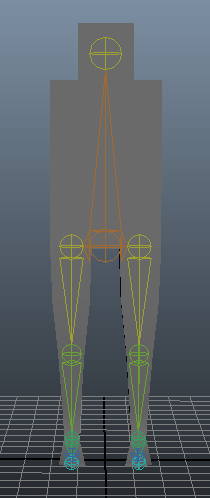
\includegraphics[height=5in]{skel_example/skel2.png}
			\caption{Example Model and Rig.  The model lacks definition for the upper body in its skeleton as the main focus is activity of the lower body as well as overall body position.}
		\end{figure}

        Simulation based character controllers offer a method to automate this process, producing animations for a character based on physical properties.  This allows for more flexible, varied animations which adjust to their environment.  Complexity of these controllers vary, but by working given starting conditions and resulting in end conditions with specified interim conditions for termination if the controller is unable to operate partway through. \cite{composable_controllers, anim_human_athletics}

\end{minipage}
\hfill
\begin{minipage}[t]{17in}
    \section*{Implementation}
        Implementation in C\# using Unity3D.

		\begin{figure}
			\centering
            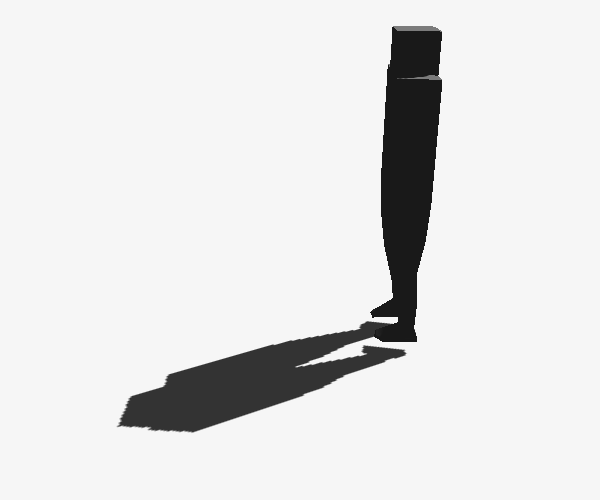
\includegraphics[width=0.2\columnwidth]{jump_sequence/jump1Cropped.png}
            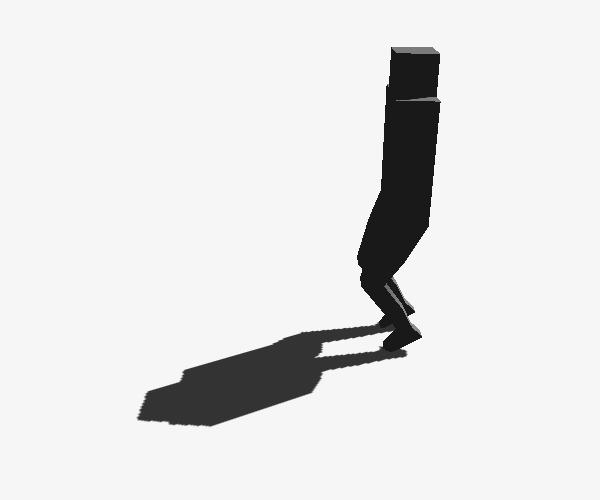
\includegraphics[width=0.2\columnwidth]{jump_sequence/jump2Cropped.png}
            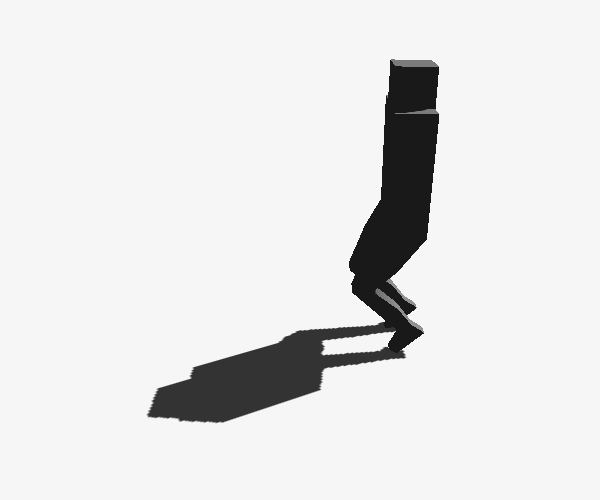
\includegraphics[width=0.2\columnwidth]{jump_sequence/jump3Cropped.png}
            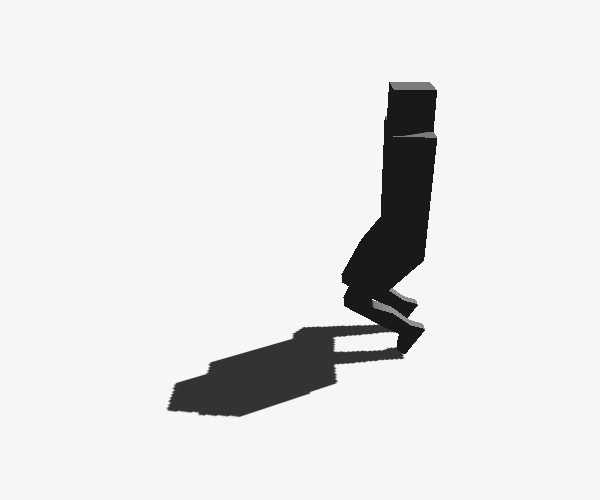
\includegraphics[width=0.2\columnwidth]{jump_sequence/jump4Cropped.png}
            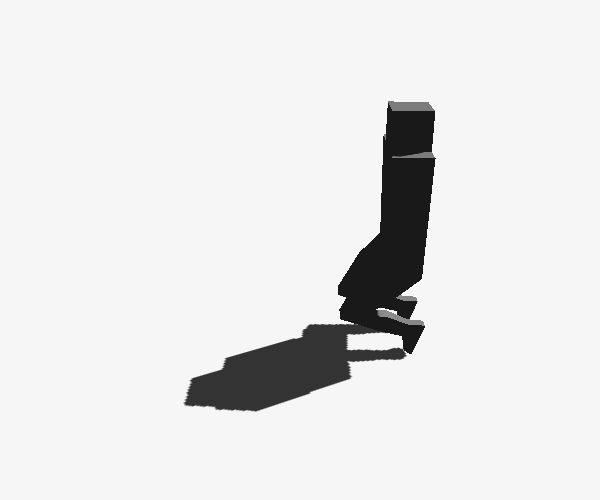
\includegraphics[width=0.2\columnwidth]{jump_sequence/jump5Cropped.png}
            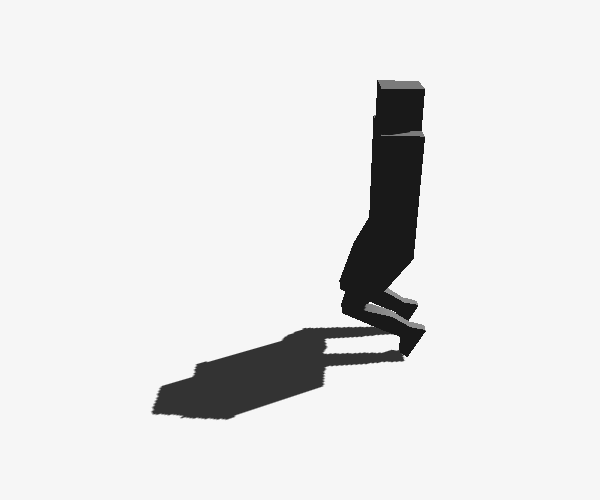
\includegraphics[width=0.2\columnwidth]{jump_sequence/jump6Cropped.png}
            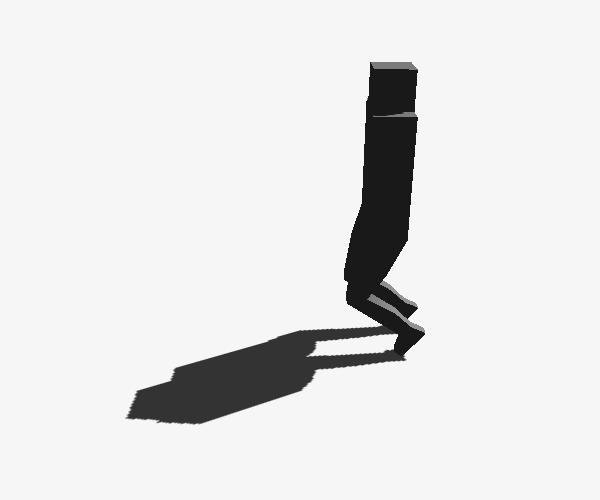
\includegraphics[width=0.2\columnwidth]{jump_sequence/jump7Cropped.png}
            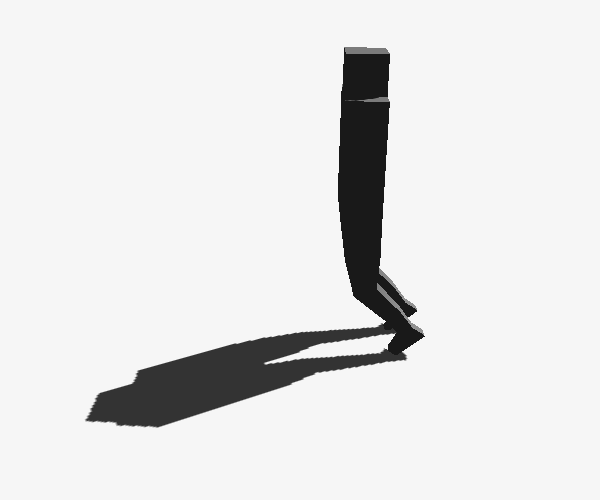
\includegraphics[width=0.2\columnwidth]{jump_sequence/jump8Cropped.png}
			\caption{Sequence of frames for a windup and acceleration for a simple human character.  Due to the focus on the lower body activity, this character lacks arms as well as complexity in its upper body skeleton.}
		\end{figure}

        \begin{figure}
            \centering
            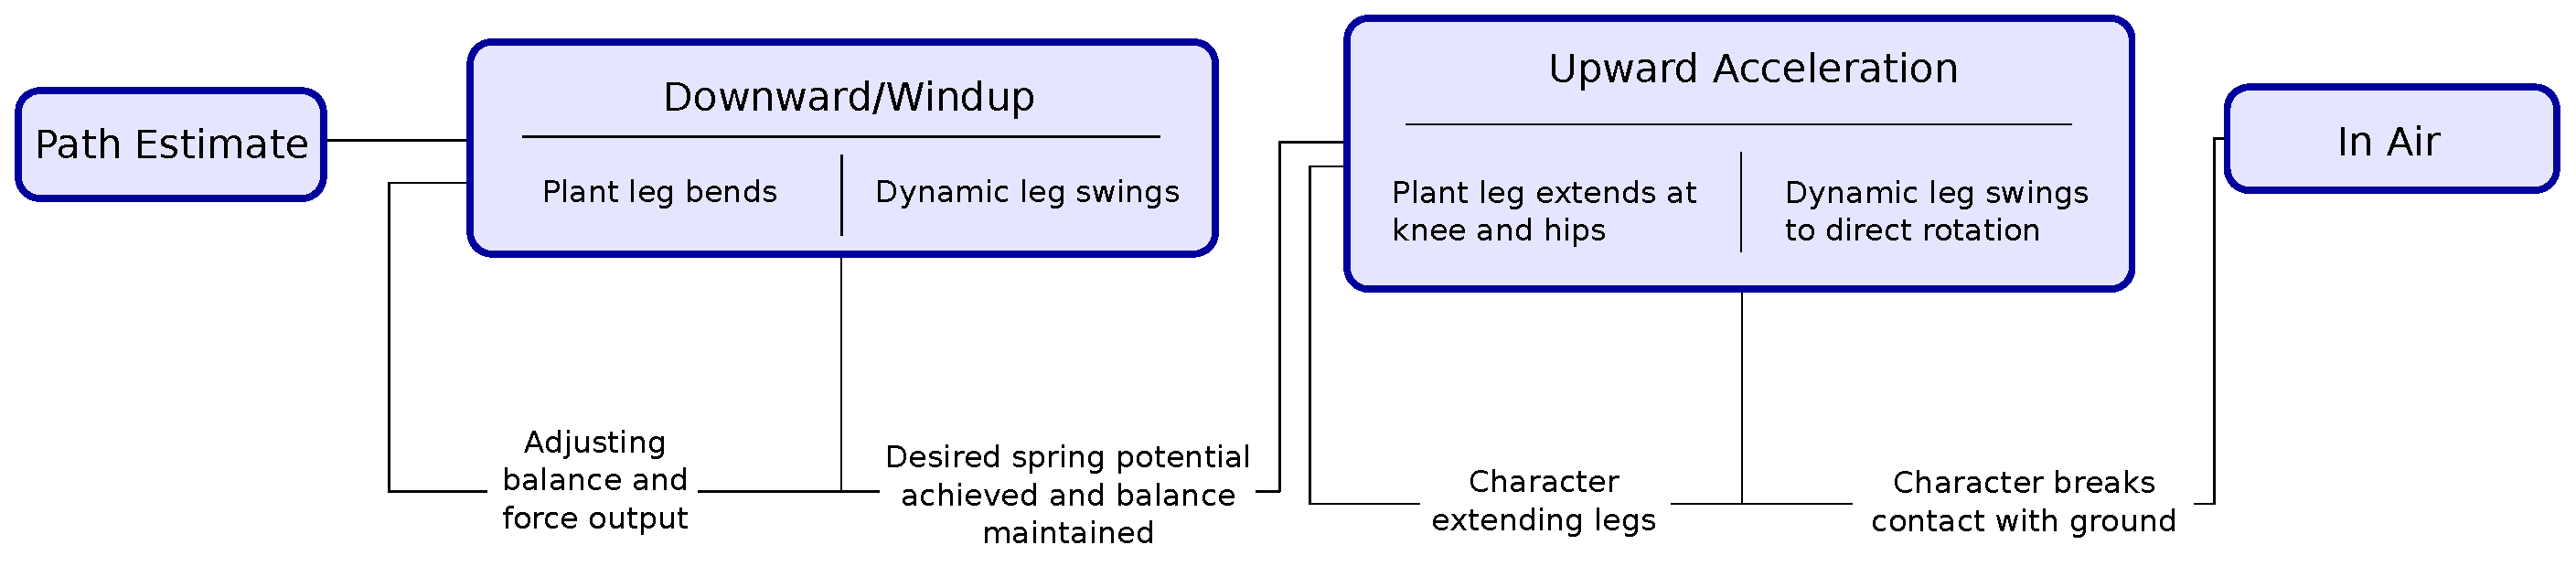
\includegraphics[width=0.8\columnwidth]{diagrams/system_diag_horiz.eps}
            \caption{The controller proceeds through the above stages, beginning with an initial calculation of the force vector required to move the character to the desired position given start and end positions as well as initial velocity, working through a chosen jump policy to decide on time to take as well as jump height.  Next the controller finds the required angles of the joints to produce this force, modeling the muscles as simple springs anchored to two different bones across a joint which gain spring potential from stretching as the joint bends.  This is performed iteratively using a PD controller, with an error function considering positioning of the center of mass over the supporting polygon in addition to the force available in the springs.  Force of the springs is used only to find joint angles.  The character then extends, unbending the joints, progressing until the feet leave the ground and the character enters the airborne phase.}
        \end{figure}

        Specifically, spring force calculations are performed using simple Hookean springs obeying \[ \vec{F} = k\vec{x} \] where $\vec{F}$ is the force of the spring, k is the spring constant, and $\vec{x}$ is the displacement of the spring from its relaxed position.  While fully muscle based models utilize spring forces in a similar, though more complex, setup to move the model using generated forces, we use the springs indirectly to calculate required joint angles, given by the force produced when a spring is stretched via the bending of the joint it crosses. \[\theta = cos^{-1} \left( ( \dfrac{2 k^2 r^2}{F^2} - 1 \right)\] This assumes that when fully extended the spring is at rest, calculating the extension of the spring as stretching over the gap or distance opened between ends of bones meeting at the joint when the joint is bent.  This distance is calculated as if the ends of bones are flat and the rotation of the joint happens at the opposite end of the split as seen in Figure \ref{fig:bone_diag}.  Modeling the muscle as such also gives the spring a $k$ which reflects the muscle when activated, assuming either full activation or a certain set activation.

\end{minipage}
%
\hfill
%%%%%%%%%%%%%%%%%%%%%%%%%%%%%%%%%%%%%%%%%%%%%%%%%%%%%%%%%%%%%%%%%%%%%%%%%%%%%%%%%%%%%%%
\begin{minipage}[t]{14in}
	\section*{Control and Visualization}
		Calculations are performed iteratively using Proportional-Derivative control, which modify value based off of the error between the current and the desired values.  This allows changes to be made to both maintain balance, which is described as distance from the center of mass to the center of the supporting polygon when projected downwards onto the plane of the supporting polygon.

        Visualization is performed using Unity3D, utilizing colored markers to track joints through the scene as well as a colored polygon to show the supporting polygon.  A simple human model is used to show the overall body position.

        \begin{figure}
			\centering
            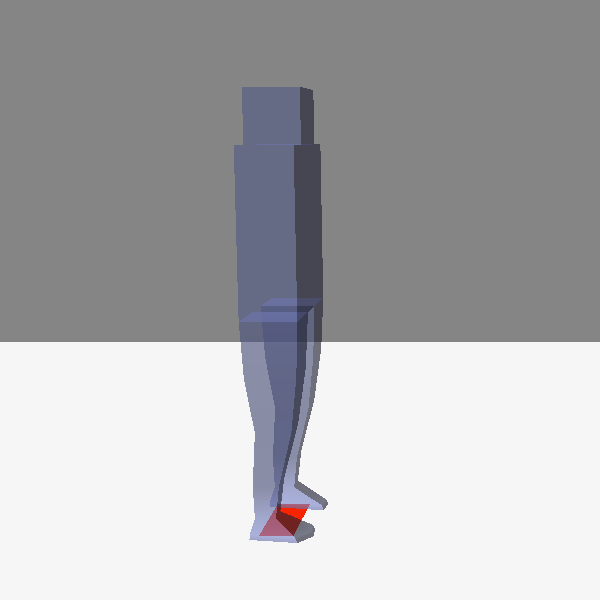
\includegraphics[width=0.15\columnwidth]{visualization/supporting_plane.png}
            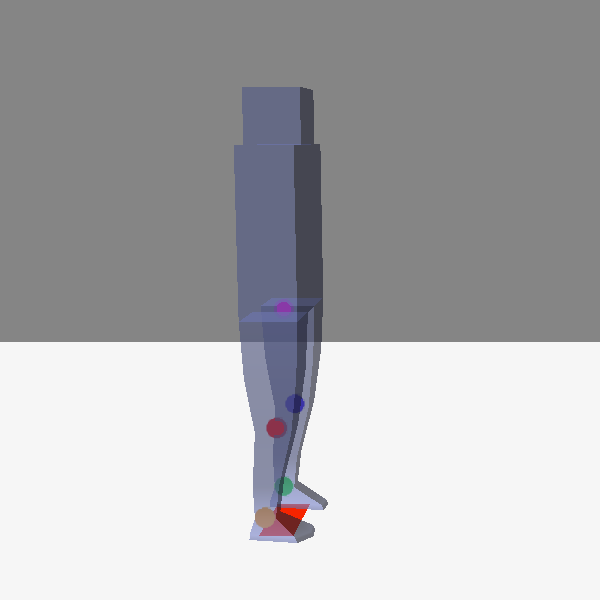
\includegraphics[width=0.15\columnwidth]{visualization/particles1.png}
            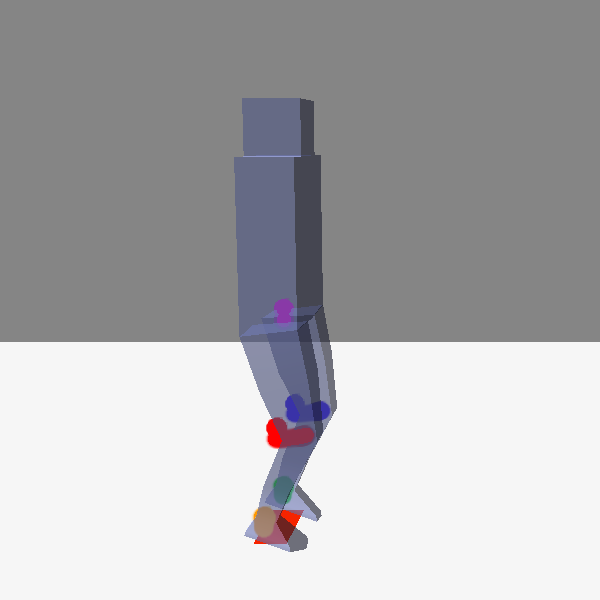
\includegraphics[width=0.15\columnwidth]{visualization/particles2.png}
            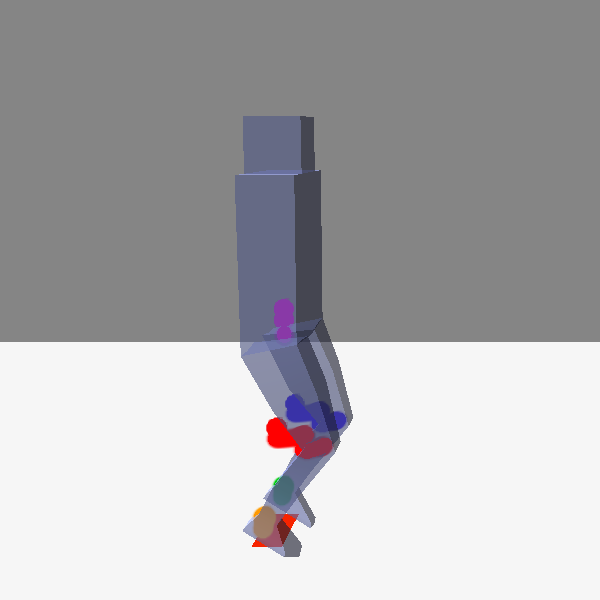
\includegraphics[width=0.15\columnwidth]{visualization/particles3.png}
            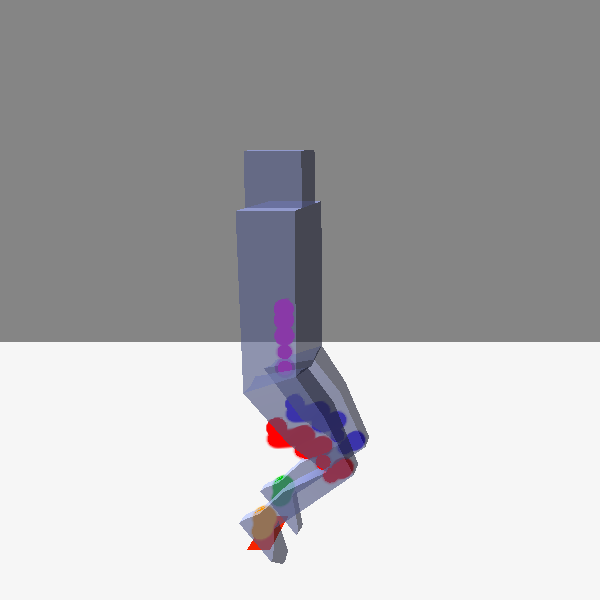
\includegraphics[width=0.15\columnwidth]{visualization/particles4.png}
            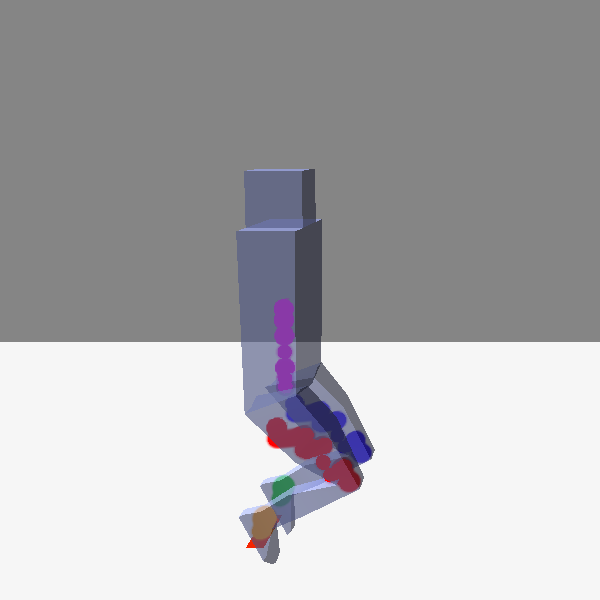
\includegraphics[width=0.15\columnwidth]{visualization/particles5.png}
			\caption{A sequence of images for a windup of the character with visualizations of joint positions and the supporting plane.  Joints tracked are the hip (purple), left and right knee (blue and red resp.), and left and right ankle (green and orange resp.).  The supporting plane is shown as a red rectangle at the feet.  Tracked joints and colors can be changed through the Unity3D inspector.}
		\end{figure}

	\section*{Future Work}
        Further work is underway to allow for more flexible starting conditions such as a running start.  Currently there is some flexibility allowing for previous velocity to be considered for force calculations, but control of the body using leg swings has yet to be implemented.

        Another desirable addition would be to take a more complex muscle system into account.  The current muscle model was chosen due to simplicity as an initial step, but ignores many factors which affect force output such as found in \cite{muscle_based_bipeds} which would aid in plausibility and accuracy.

        Additional controllers could be also combined with this to produce complex motions such as parkour vaults and flips, which are becoming more prevalent in both films and video games.  This would also require the controller to take more complex skeletons into account, utilizing arms and upper body movement more.  These controllers would focus mainly on the in-air and landing phases to produce more motions as found in existing work on controllers. \cite{falling_landing, composable_controllers, anim_human_athletics}

        %Finally, the current implementation utilizes a highly simplified model of force application.  Torque should be taken into account, allowing the force assignment to be performed as a maximum flow problem, as well as more accurately describing the force contribution of each muscle group to the movement of the body.  Capacity for joints could be given by the arc traced by the bone primarily affected by the joint when fully extended and fully flexed.
		
	\vspace{0.2in}

	{\footnotesize
	\bibliographystyle{abbrv}
    \nocite{muscle_based_bipeds}
    \nocite{anim_human_athletics}
    \nocite{composable_controllers}
    %\nocite{soft_contacts}
    \nocite{falling_landing}
    %\nocite{vball_footwork_block}
    %\nocite{static_block_jumps}
    %\nocite{inter_physics_anim}
    %\nocite{opt_motion_synth}
    %\nocite{motion_intentions}
    %\nocite{block_spike_survey}
    %\nocite{robust_ctrl_policies}
    %\nocite{automatic_gait}
    %\nocite{humanoid_robots_jump}
    %\nocite{cat_hindlimb_activity}
    %\nocite{cat_thigh_activity}

    \begin{figure}
        \label{fig:bone_diag}
        \centering
        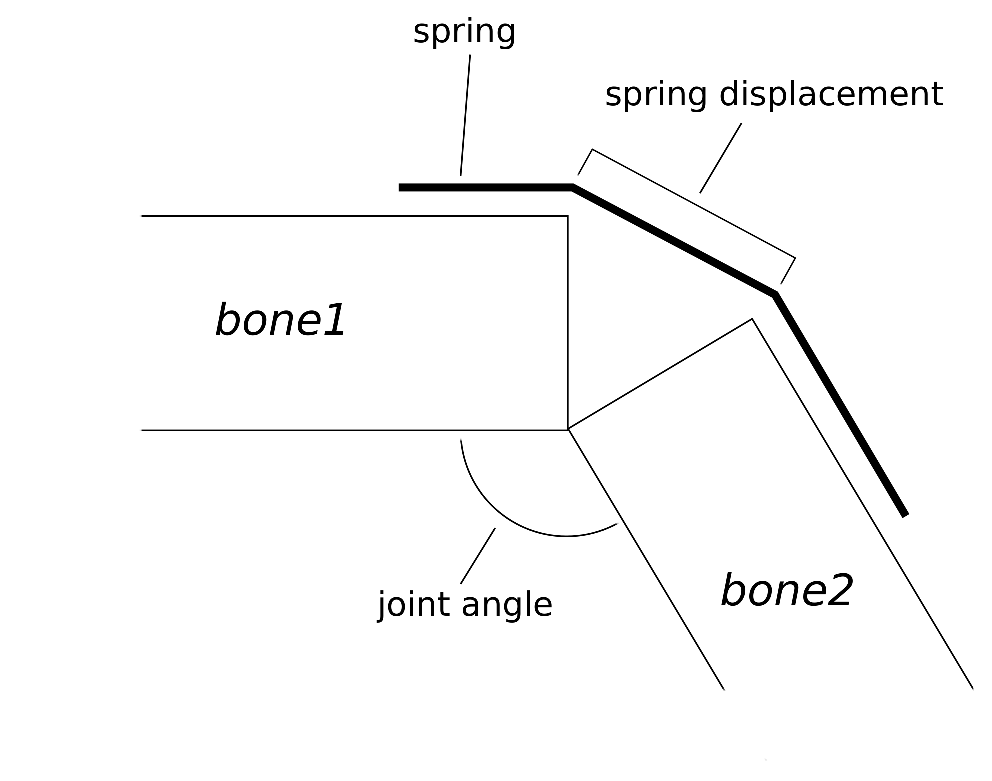
\includegraphics[height=2in]{diagrams/spring_angle_calc.eps}
        \caption{Diagram of the spring extension over ends of bones.}
    \end{figure}

	\bibliography{refs}
	}
\end{minipage}
%%%%%%%%%%%%%%%%%%%%%%%%%%%%%%%%%%%%%%%%%%%%%%%%%%%%%%%%%%%%%%%%%%%%%%%%%%%%%%%%%%%%%%%
%%%%%%%%%%%%%%%%%%%%%%%%%%%%%%%%%%%%%%%%%%%%%%%%%%%%%%%%%%%%%%%%%%%%%%%%%%%%%%%%%%%%%%%

\end{document}

